\chapter{Doświadczenie}
Przeprowadzone doświadczenie polega na porównaniu dostępnych w środowisku Microsoft Azure algorytmów klasyfikacji danych dwu-klasowych wraz z algorytmem stworzonym na potrzeby pracy inżynierskiej o tytule ''\textit{Wykorzystanie algorytmów genetycznych w systemach wykrywania intruzów w sieciach komputerowych}''\cite{Blyszcz2022} oraz z algorytmem DANet\cite{Chen2022}. Doświadczenie przebiegało według \refsource{schematu}{fig:sch-prac}.

\begin{figure}[H]
    \centering
    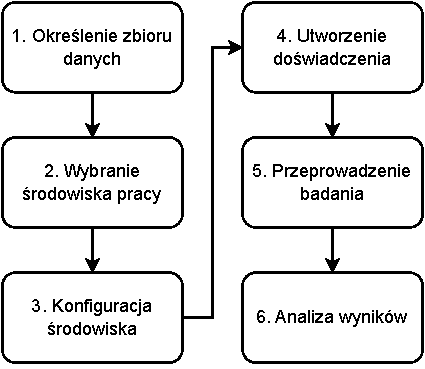
\includegraphics[width=0.9\textwidth]{images/schemat_pracy}
    \captionsource{Schemat przebiegu doświadczenia}{Opracowanie własne}
    \label{fig:sch-prac}
\end{figure}

\section{Metodologia badwcza}
Przyjęta w projekcie metodologia badawcza została określona w poniższej \refsource{tabeli}{tab:met-bad}. Przyjęta metodologia ma za zadanie określić jakoś porównywanego algorytmu.

\begin{table}[H]
    \centering
    \captionsource{Metodologia badawcza}{Opracowanie własne}
    \begin{tabular}{|L{\textwidth}|}
        \hline
        \textbf{Problem badawczy:} \\
        Czy algorytm klasyfikacji danych utworzony w ramach pracy inżynierskiej może konkurować z rozwiązaniami dostępnymi w środowiskach komercyjnych \\ \hline

        \textbf{Pytania badawcze:} \\
        \begin{enumerate}
            \item Czy algorytm jest konkurencyjny pod względem wybranych metry:
            \begin{itemize}
                \item dokładność algorytmu
                \item czas działania
                \item precyzja
                \item czułość
                \item f1
                \item auc
            \end{itemize}
        \end{enumerate} \\ \hline

        \textbf{Hipotezy:} \\
        \begin{enumerate}
            \item Nie ma istotnej różnicy w uzyskanej ''\textit{dokładności}'' między algorytmami.
            \item Nie ma istotnej różnicy w uzyskanej ''\textit{czułości}'' między algorytmami.
            \item Nie ma istotnej różnicy w uzyskanej ''\textit{precyzji}'' między algorytmami.
            \item Nie ma istotnej różnicy w uzyskanym ''\textit{auc}'' między algorytmami.
            \item Nie ma istotnej różnicy w uzyskanej ''\textit{f1}'' między algorytmami.
            \item Nie ma istotnej różnicy w uzyskanym ''\textit{czasie działania}'' między algorytmami.
        \end{enumerate} \\ \hline
    \end{tabular}
    \label{tab:met-bad}
\end{table}

\section{Dane}
Zbiór danych został przygotowany przez Kanadyjski Instytut Cyberbezpieczeństwa działający przy Uniwersytecie Nowy Brunszwik za pomocą narzędzia CICFlowMeter\cite{Ahlashkari2022}. Zbiór zawiera 79 cech ruchu sieciowego do których zaliczyć można: etykietę, czas trwania przesyłu, minimalną długość pakietu zwrotnego, maksymalną długość pakietu zwrotnego, port docelowy, długość pakietów. Zbiór pozwala na określenie czy ruch sieciowy jest życzliwy \trans{ang. BENING}, czy nieżyczliwy (różne możliwe formy ataku na sieć). Dodatkowo zbiór został podzielony na pięć dni roboczych: poniedziałek 3.07.2017 - piątek 7.07.2017. Dane z poniedziałku zawierają jedynie ruch życzliwy, zaś w pozostałe dni zostały zasymulowane ataki na sieć komputerową\cite{Blyszcz2022, unbkaggle}.

\section{Środowisko programistyczne}
Jako środowisko programistyczne zostało wybrane Azure Machine Learning Studio z powodu możliwości uniezależnienia obliczeń od komputera lokalnego, dodatkowo platforma umożliwia łatwy sposób na tworzenie skomplikowanych potoków zadań, które składają się z komponentów wielokrotnego użytku. Każdy komponent uruchamia się w środowisku odizolowanym od pozostałych operacji. Dzieje się tak dzięki wykorzystaniu wielo węzłowych klastrów obliczeniowych, bazujących na oprogramowaniu Docker, klastry te mogą skalować się w zależności od potrzeb oraz dostępnej jednostki\cite{MicrosoftLearn2023}.
\\ \\
Całe doświadczenie zostało odwzorowane w graficznym potoku narzędzia ''\textit{Projektant}'' oraz przedstawione na \refsource{zdjęciu}{fig:pipeline}.

\begin{landscape}
\begin{figure}[H]
    \centering
    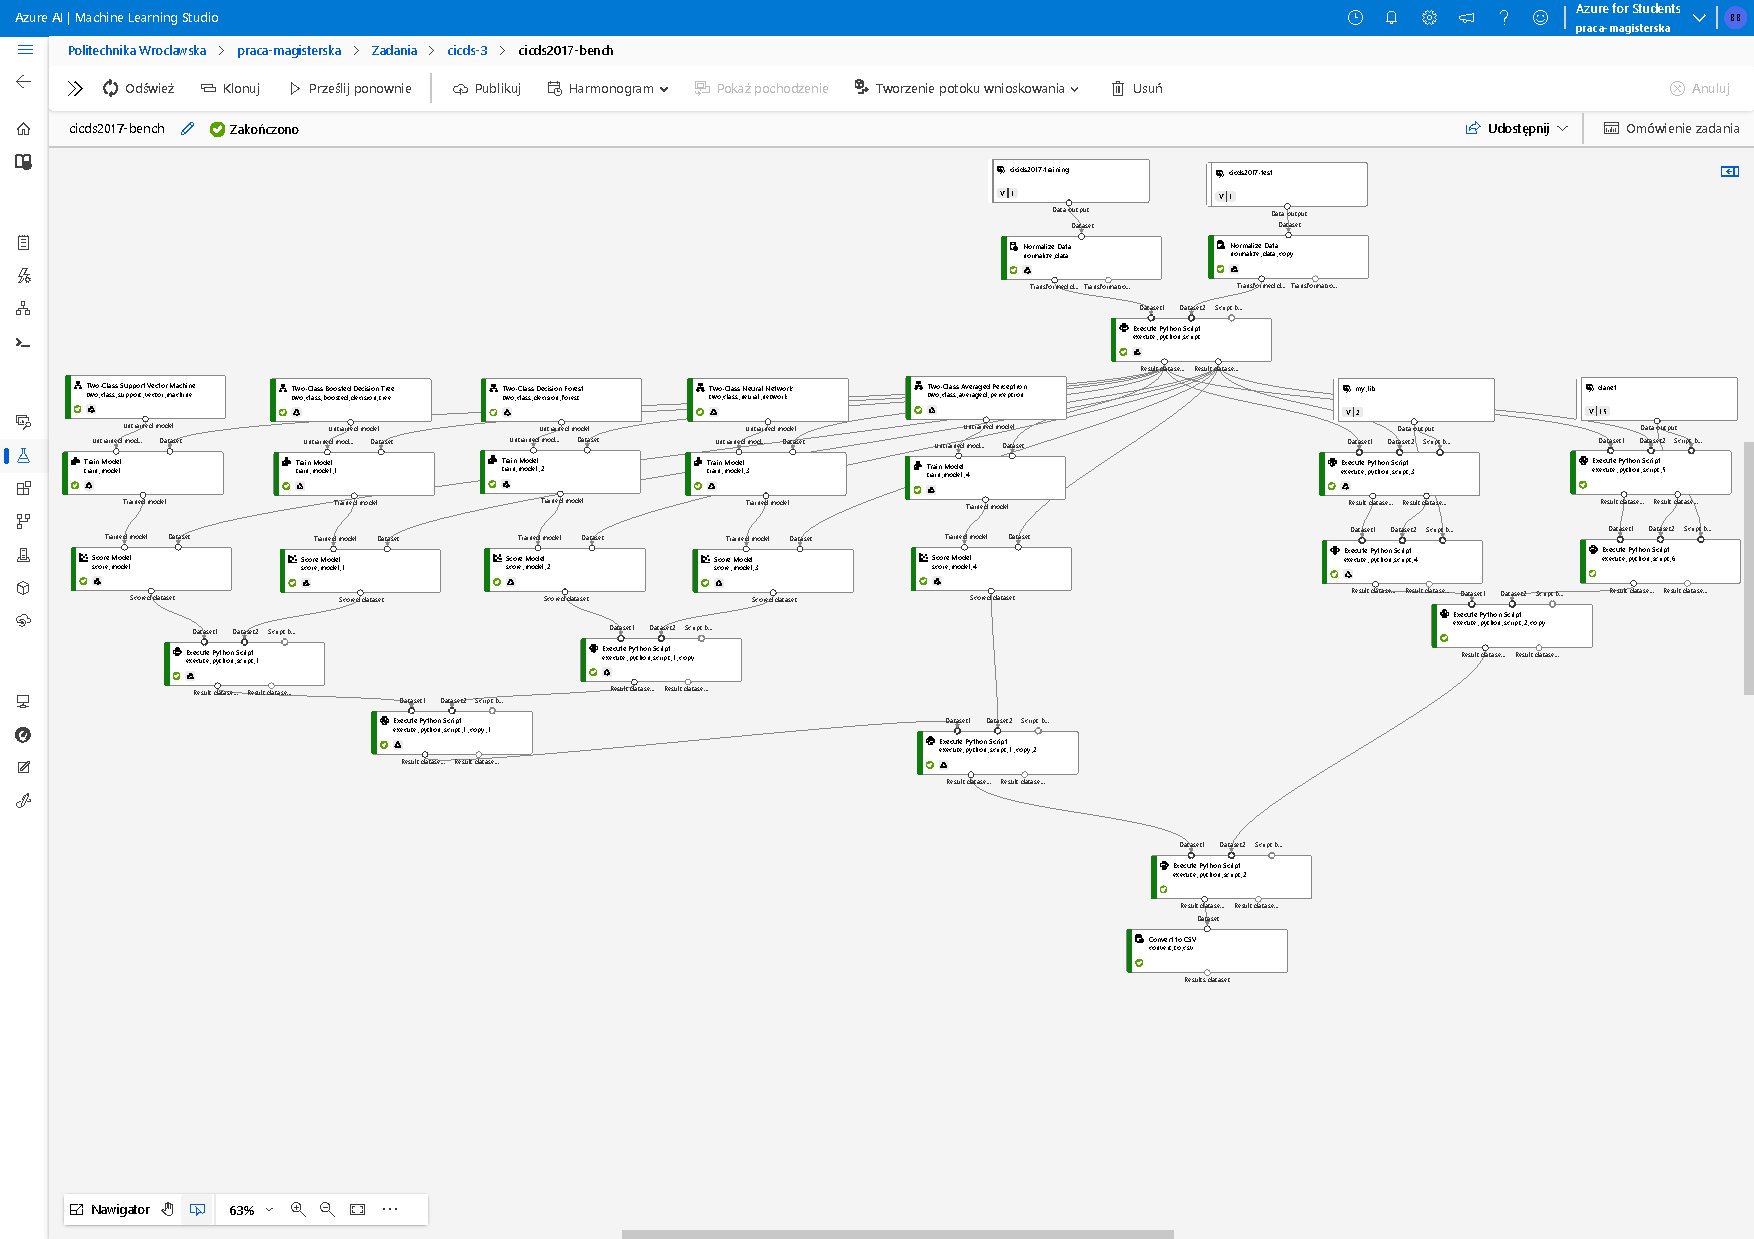
\includegraphics[height=0.9\textwidth]{images/pipeline}
    \captionsource{Potok zadań}{Opracowanie własne}
    \label{fig:pipeline}
\end{figure}
\end{landscape}

\section{Algorytmy}

\subsection{Two-Class Support Vector Machine}
\begin{figure}[H]
    \centering
    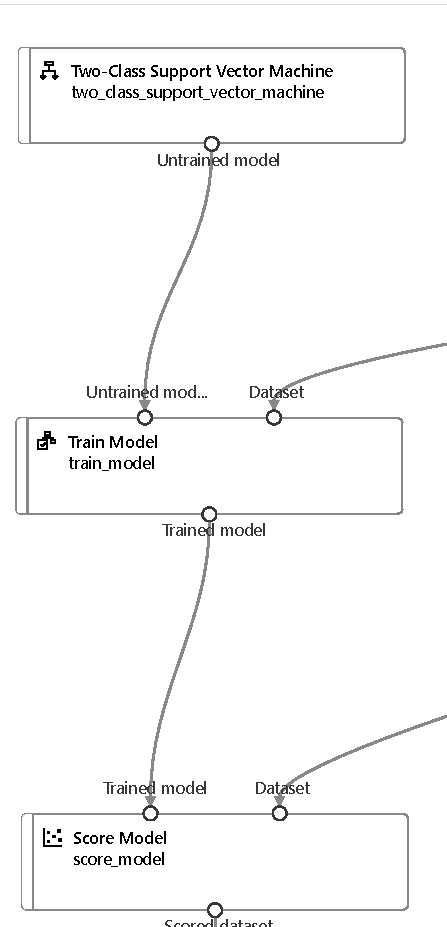
\includegraphics[width=0.4\textwidth]{images/svm_pipe}
    \captionsource{Potok zadań dla modelu \textit{Two-Class Support Vector Machine}}{Opracowanie własne}
    \label{fig:svm-pipe}
\end{figure}

\subsection{Two-Class Boosted Decision Tree}
\begin{figure}[H]
    \centering
    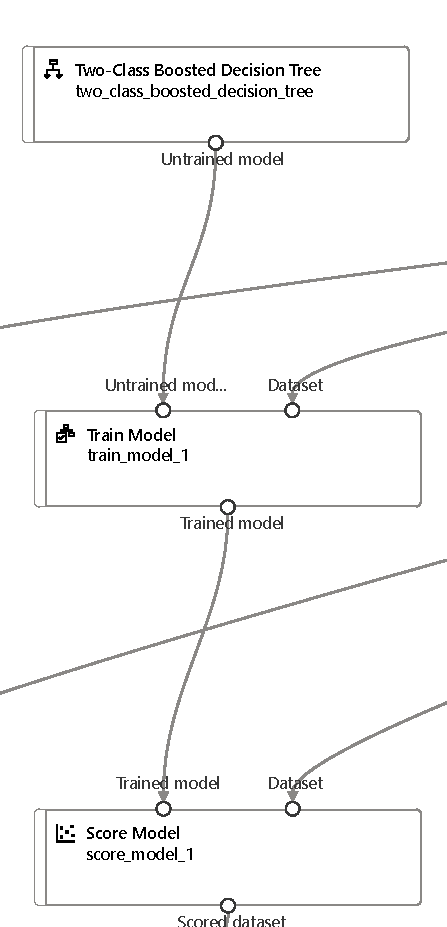
\includegraphics[width=0.4\textwidth]{images/dt_pipe}
    \captionsource{Potok zadań dla modelu \textit{Two-Class Boosted Decision Tree}}{Opracowanie własne}
    \label{fig:dt-pipe}
\end{figure}

\subsection{Two-Class Decision Forest}
\begin{figure}[H]
    \centering
    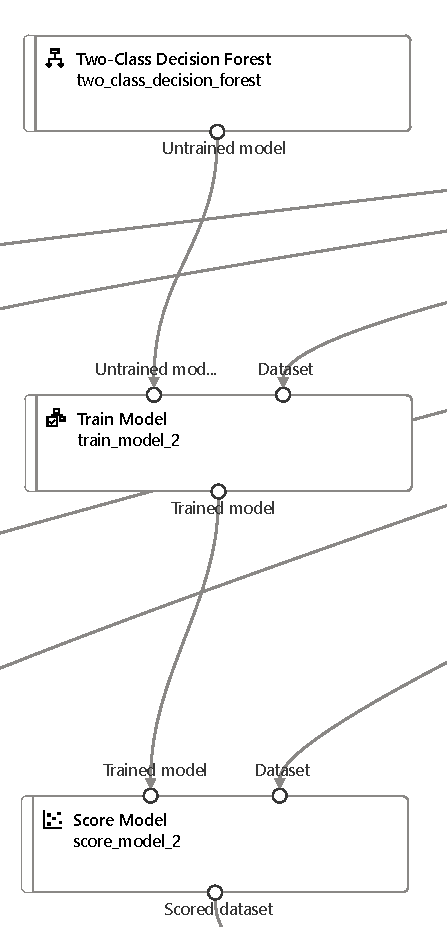
\includegraphics[width=0.4\textwidth]{images/df_pipe}
    \captionsource{Potok zadań dla modelu \textit{Two-Class Decision Forest}}{Opracowanie własne}
    \label{fig:df-pipe}
\end{figure}

\subsection{Two-class Neural Network}
\begin{figure}[H]
    \centering
    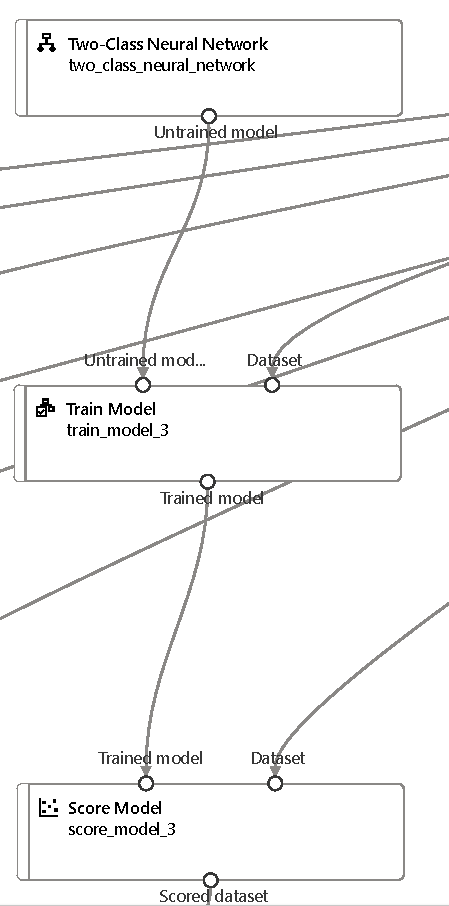
\includegraphics[width=0.4\textwidth]{images/nn_pipe}
    \captionsource{Potok zadań dla modelu \textit{Two-Class Neural Network}}{Opracowanie własne}
    \label{fig:nn-pipe}
\end{figure}

\subsection{Two-Class Average Perceptron}
\begin{figure}[H]
    \centering
    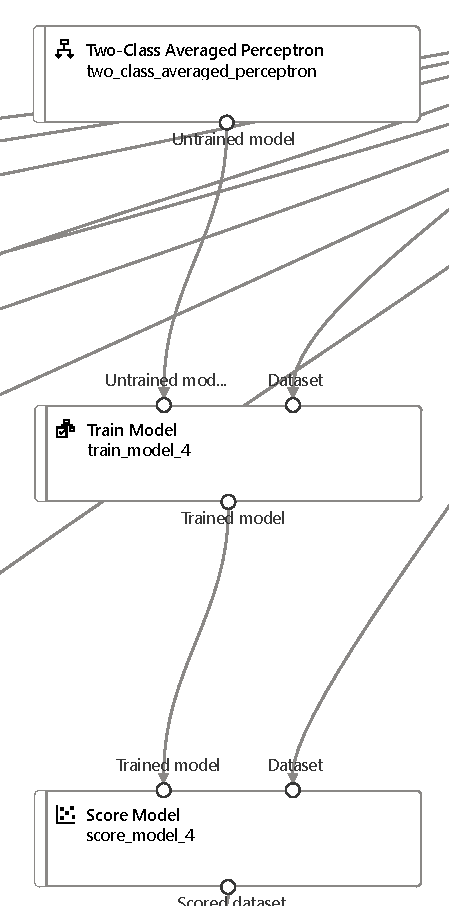
\includegraphics[width=0.4\textwidth]{images/ap_pipe}
    \captionsource{Potok zadań dla modelu \textit{Two-Class Average Perceptron}}{Opracowanie własne}
    \label{fig:ap-pipe}
\end{figure}

\subsection{Autorskie rozwiązanie}
\begin{figure}[H]
    \centering
    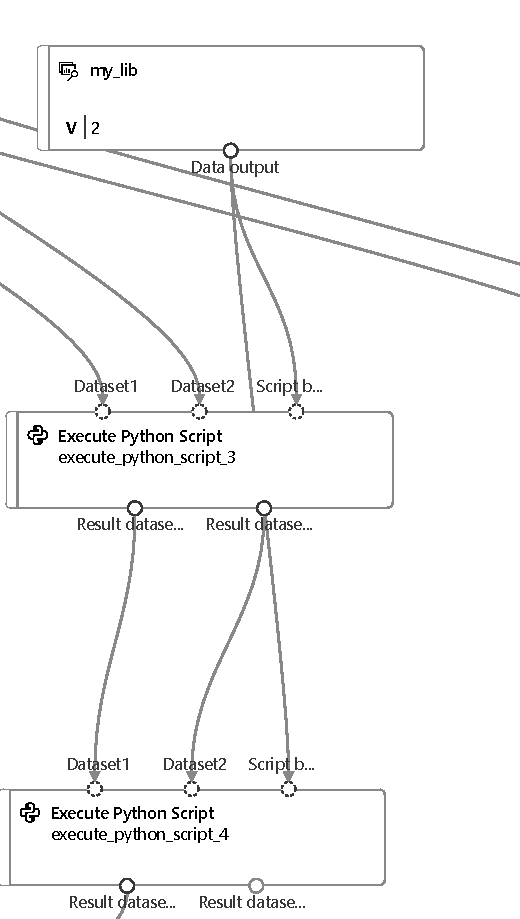
\includegraphics[width=0.4\textwidth]{images/ga_pipe}
    \captionsource{Potok zadań dla modelu}{Opracowanie własne}
    \label{fig:ga-pipe}
\end{figure}

\subsection{DANet}
\begin{figure}[H]
    \centering
    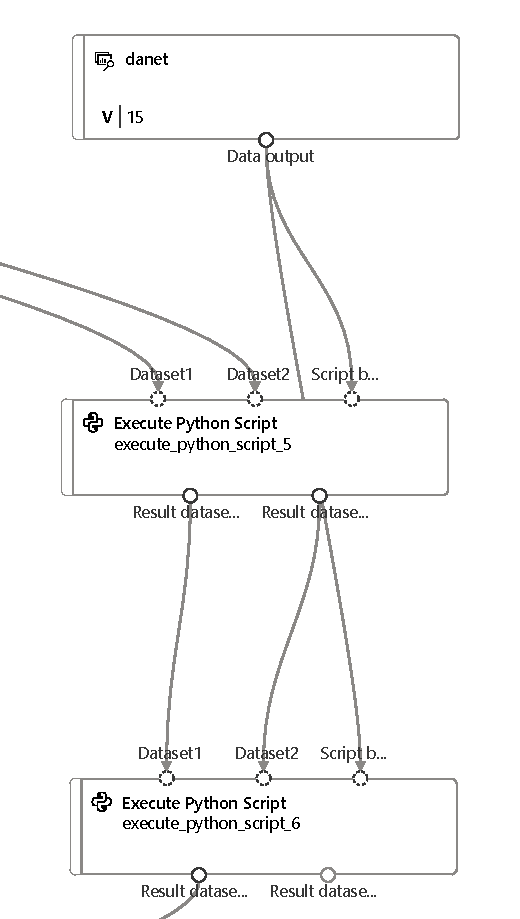
\includegraphics[width=0.4\textwidth]{images/danet}
    \captionsource{Potok zadań dla modelu \textit{DANet}}{Opracowanie własne}
    \label{fig:danet-pipe}
\end{figure}




